\section{Overview}

\subsection{Agency}

\begin{enumerate}
    \item Ask: is the principal liable to a third party for another's actions?
    \item \textbf{Three actors}: principal, agent, third party. The third 
    party is bringing the claim.
    \item Two types of cases: \textbf{contract} and \textbf{tort}.
    \item Is there an \textbf{agency relationship}? Elements:\footnote{See 
    Restatement (Third) \S\ 1.01. This step of the analysis applies to both 
    contract and tort cases.}
    \begin{enumerate}
        \item The principal's \textbf{manifestation of assent}. (This can 
        exist even if the principal explicitly denies an agency relationship. 
        The terminology of the agreement is not controlling.\footnote{Casebook 
        p. See, e.g., \emph{Cargill}, where the lawyers disclaimed an agency 
        relationship in the initial agreement.})
        \item Agent acting on the principal's \textbf{behalf}. (Do the agent's 
        actions directly benefit the principal?)
        \item Agent subject to the principal's \textbf{control}.
        \item Agent \textbf{consents}.
        \item Examples:
        \begin{enumerate}
            \item Setting the \textbf{purpose and conditions} of activity can 
            establish an agency relationship. \emph{Gorton v. Doty}, p.  
            \pageref{subsub:gorton}.
            \item A creditor that exercises enough control over a debtor's 
            business can be liable as a principal for the debtor's acts. 
            \emph{A. Gay Jenson Farms Co. v. Cargill}, p. 
            \pageref{subsub:cargill}.
        \end{enumerate}
    \end{enumerate}
    \item If this is a \textbf{breach of contract} case:
    \begin{enumerate}
        \item Did the agent have \textbf{authority} to act? Types of authority 
        (which often overlap):\footnote{This step applies \emph{only} to 
        contract cases.}
        \begin{enumerate}
            \item \textbf{Actual}: can be (1) express or (2) implied. \S\S\ 
            2.01--2.02.
            \item \textbf{Apparent}: did the third party reasonably believe 
            the agent had authority, and was that belief \emph{traceable} to 
            the principal's manifestations? \S\ 2.03.
            \item (These often overlap---e.g., \emph{Mill Street Church}, p.  
            \pageref{par:mill}.)
        \end{enumerate}
        \item Do any \textbf{exceptions} apply?\footnote{These are substitutes 
        for authority.}
        \begin{enumerate}
            \item \textbf{Ratification}: requires the principal's (1) 
            \textbf{intent to ratify} and (2) \textbf{full knowledge} of 
            material circumstances. \emph{Botticello v. Stefanovicz}, p.  
            \pageref{par:botticello}. See also Restatement (Third) \S\S\ 4.01 
            (definition), 4.02 (effect), and 4.05(1) (timing).
            \item \textbf{Estoppel}: a third party can assert estoppel when 
            he (1) \textbf{detrimentally relies} on an impostor agent and (2) 
            the principal \textbf{intentionally or carelessly} caused the 
            belief or the principal \textbf{was on notice} and failed to take 
            reasonable steps. Restatement (Third) \S\ 2.05 and 
            \emph{Hoddeson}, p. \pageref{par:hodd}.
            Estoppel only creates liability for the 
            principal (i.e., the principal can't assert estoppel against the 
            third party).
            \item \textbf{Undisclosed principal}: if the agent lacks 
            authority (either actual or apparent), the undisclosed principal 
            can still be liable for acts that are ``within the authority 
            usually confided'' to agents. See \emph{Watteau}, p. 
            \pageref{par:watteau}. Requires an underlying agency 
            relationship.
        \end{enumerate}
    \end{enumerate}
    \item If this is a \textbf{tort} case:
    \begin{enumerate}
        \item \textbf{Respondeat superior}: employers are liable for torts 
        their \textbf{employees} commit while within the \textbf{scope of 
        employement}. Restatement (Third) \S\ 2.04.
        \begin{enumerate}
            \item \textbf{Definition of employee}: is an agent (under 
            Restatement \S\ 1), and the principal controls or has the right to 
            control the \textbf{manner and means} of the work. Restatement 
            (Third) \S\ 7.07(3).
            \begin{enumerate}
                \item Servant/employee: principal is liable for torts if the 
                employee was acting within the scope of employment.
                \item Independent contractor (agent-type): P is liable for 
                contracts but not torts.
                \item Independent contractor (non-agent): P is not liable.
            \end{enumerate}
            \item \textbf{Definition of scope of employement}: doesn't include 
            independent courses of conduct not intended to serve the 
            employer's purposes. Restatement (Third) \S\ 7.07.  
            \end{enumerate}
        \item \textbf{Exceptions} (under which P is liable):
        \begin{enumerate}
            \item Engaging an incompetent contractor.
            \item Nondelegable duty.
        \end{enumerate}
        \item \textbf{Employees vs. independent contractors} (Restatement 
        (Second) \S\ 220(2)):
        \begin{enumerate}
            \item P \emph{may} exercise control over details of A’s work
            \item A does not engage in distinct business
            \item Type of work typical of supervised employee, not unsupervised specialist
            \item Job requires low skill level
            \item P supplies tools and dictates place of work
            \item A employed for a long term
            \item A is compensated by time and not by job
            \item Work is a regular part of P’s business
            \item Intent to create employer/employee relationship
            \item P is in business
            \item See gas station cases (\emph{Humble} and \emph{Sun Oil}) for 
            similar facts reaching different conclusions on the 
            employee-vs.-independent-contractor question.
        \end{enumerate}
        \item \textbf{Franchises}: a standard franchise system does not 
        necessarily establish an employee relationship (\emph{Murphy}), but it 
        can if the franchisees are tightly controlled (\emph{McDonald's).}
        \item \textbf{Apparent authority}: arises when the principal 
        represents that another is his servant or other agent and causes the 
        third person to rely upon the \textbf{care or skill} of the apparent 
        agent. Does not require an agency relationship under \S\ 1. 
        \emph{McDonald's}.
        \begin{enumerate}
            \item Why is this different than apparent \emph{agency}? Because 
            authority doesn't apply to tort cases. Torts are about 
            \emph{mistakes}, not \emph{instructions}. Principals rarely 
            authorize their agents to commit torts.
        \end{enumerate}
    \end{enumerate}
    \item \textbf{Agent liability}:
    \begin{enumerate}
        \item A is liable for his own torts.
        \item A is liable in contract when:
        \begin{enumerate}
            \item Acting without authority (because of the implied warranty).
            \item When acting for an undisclosed or unidentified principal.
        \end{enumerate}
        \item A is liable to the principal for breach of fiduciary duty.
    \end{enumerate}
    \item \textbf{Agent's fiduciary duties}:
    \begin{enumerate}
        \item Loyalty.
        \begin{enumerate}
            \item Material benefit arising out of position.
            \item Acting as or on behalf of adverse party.
            \item Competition.
            \item Use of principal's property \& confidential info.
        \end{enumerate}
        \item Care, competence, and diligence.
        \item Act within scope of authority.
    \end{enumerate}
    \item \textbf{Strategies for avoiding liability}:
    \begin{enumerate}
        \item (First, define the \textbf{risks and rewards}.)
        \item Get \textbf{insurance}. \emph{Gorton v. Doty}, p.
        \pageref{subsub:gorton}.
        \item \textbf{Legal structuring}: structure the relationship to negate 
        one of the four elements.
        \begin{enumerate}
            \item Specify the nature of the relationship, ideally in writing.
            \item Delegate control to another principal, or give up control 
            entirely.
        \end{enumerate}
        \item \textbf{Security/collateral}. E.g., a right of first refusal. 
        \emph{A. Gay Jenson Farms Co. v. Cargill}, p.  
        \pageref{subsub:cargill}. \emph{Cargill}.
        \item \textbf{Monitoring}. E.g., accounting audits.
        \item \textbf{Operational control}. E.g., a sign-off requirement for 
        major decisions. \emph{Cargill} again.
        \item \textbf{Due diligence}. E.g., verify the type of property 
        interest that the seller is selling. \emph{Botticello v. Stefanovicz}, 
        p. \pageref{par:botticello}.
        \item \textbf{Recording/registration systems}. E.g., check public land 
        records. \emph{Botticello}.
    \end{enumerate}
    % Include Cable chart
    \includepdf{resources/agency.pdf}
\end{enumerate}

\newpage

\subsection{Partnership}

\begin{enumerate}
    \item \textbf{What is a partnership and who are the partners?}
    \begin{enumerate}
        \item ``The association of two or more persons to carry on as 
        co-owners a business for profit forms a partnership, whether or not 
        the persons intended to form a partnership.'' RUPA \S\ 202(a)
        \item \textbf{Profit sharing} and \textbf{management rights} weigh in 
        favor of the existence of a partnership. But profit sharing alone 
        without sharing in losses is not enough to establish a partnership. 
        \emph{Fenwick}, p. \pageref{par:fenwick-ucc}.
        \item The partners' \textbf{intent} is not determinative.
        \item All partners are \textbf{jointly and severally liable} for all 
        obligations of the partnership. RUPA \S\ 305.
        \item Partnership by \textbf{estoppel}:
        \begin{enumerate}
            \item \textbf{Representation/holding out} that one person is the 
            partner of another.
            \item Representation came from the \textbf{defendant}.
            \item Plaintiff \textbf{relied}, reasonably and in good faith, on 
            the representation.
            \item The plaintiff suffered a \textbf{detrimental change in 
            position} based on that reliance.
            \item See \emph{Young v. Jones}, p. \pageref{par:young}, finding 
            no partnership by estoppel.
        \end{enumerate}
    \end{enumerate}
    \item \textbf{Partners' fiduciary duties}:
    \begin{enumerate}
        \item Partners owe a duty to other partners. \emph{Meinhard v. 
        Salmon}, p. \pageref{par:meinhard}.
        \item RUPA \S\ 404 seems to require a duty to \textbf{share} in 
        partnership opportunities.
    \end{enumerate}
    \item \textbf{Rights of partners}:
    \begin{enumerate}
        \item Each partner is an agent of the partnership with equal rights. 
        RUPA \S\S\ 301(1), 401(f). \emph{National Biscuit v. Stroud}, \pageref{par:biscuit}.
        \item Limiting one partner's authority requires a majority vote. RUPA 
        \S\ 401(j). But one partner is not a majority. Two-person partnerships 
        can end in deadlock. \emph{Summers v. Dooley}, p. 
        \pageref{par:summers}.
    \end{enumerate}
\end{enumerate}

\newpage

\subsection{Corporate Formation}

\begin{enumerate}
    \item \textbf{Corporate structure}.
    \begin{enumerate}
        \item \textbf{Public}: many public shareholders, liquid shares, traded 
        on an exchange.
        \item \textbf{Private} or \textbf{closely held}: few shareholders, 
        shareholders are also officers and directors, shares are hard to sell.
        \item \textbf{Dividens}: paid at the board's discretion.
    \end{enumerate}
    \item \textbf{Formation}.
    \begin{enumerate}
        \item \textbf{Articles of incorporation}: incorporator (often a 
        lawyer) files and then (1) organizes the company herself or (2) names 
        initial directors, who then do the rest. MBCA \S\ 2.05.
        \item \textbf{Capital structure}: authorized shares---common stock, 
        preferred stock. MBCA \S\S\ 6.01--02.
        \item \textbf{Organizational consent} (at a meeting or by written 
        consent): adopt bylaws, elect officers, conduct ``other business.'' 
        MBCA \S\ 2.05.
        \item \textbf{Bylaws}: repeat provisions from statute and articles; 
        governance procedures; officer duties and authority; rules for bylaw 
        amendments. MBCA \S\ 2.06.
        \item \textbf{Officer appointments}: few requirements, although some 
        states require president, secretary, etc. MBCA \S\ 8.40.
        \item \textbf{Stock issuance}: \textbf{subscription} (agreement to 
        purchase on specified terms) or \textbf{issuance} (ritual of 
        certificating and entering on stock register). MBCA \S\S\ 6.20--21.
        \item \textbf{Shareholders' agreement}: a private contract among 
        shareholders.
        \item \textbf{Annual election of officers and directors}, as required 
        by statute.
    \end{enumerate}
    \item \textbf{Limited liability}.
    \begin{enumerate}
        \item \textbf{Enterprise liability}:
        \begin{enumerate}
            \item Holds sister corporations liable when money, operations, and 
            employees are commingled.
            \item Good record-keeping can avoid commingling.
        \end{enumerate}
        \textbf{Piercing the corporate veil} can result from:
        \begin{enumerate}
            \item \textbf{Unity of interest and ownership} between a 
            shareholder and corporation (i.e., sloppiness):
            \begin{enumerate}
                \item Not following \textbf{formalities}; or
                \item \textbf{Commingling} corporate and personal business; or
                \item \textbf{Undercapitalization};
            \end{enumerate}
            \item Or \textbf{promotion of injustice}:
            \begin{enumerate}
                \item \textbf{Fraudulent conduc} (e.g., promising payment 
                while draining assets); or
                \item \textbf{Unjust enrichment}.
            \end{enumerate}
            \item % TODO add walkovsky -- taxi case
        \end{enumerate}
        \item \textbf{Dividend rules}:
        \begin{enumerate}
            \item Corporations must be able to \textbf{pay creditors} before 
            issuing dividends. MBCA \S\ 6.40.
            \item Directors are \textbf{personally liable} for impermissible 
            dividends. MBCA \S\ 8.33.
        \end{enumerate}
        \item \textbf{Reverse piercing}:
        \begin{enumerate}
            \item Assume no enterprise liability.
            \item Apply PVC test downward to to reach the assets of a 
            subsidiary. \emph{Sea-Land}. % TODO add xref
            % Include `deep pockets' exam review chart
            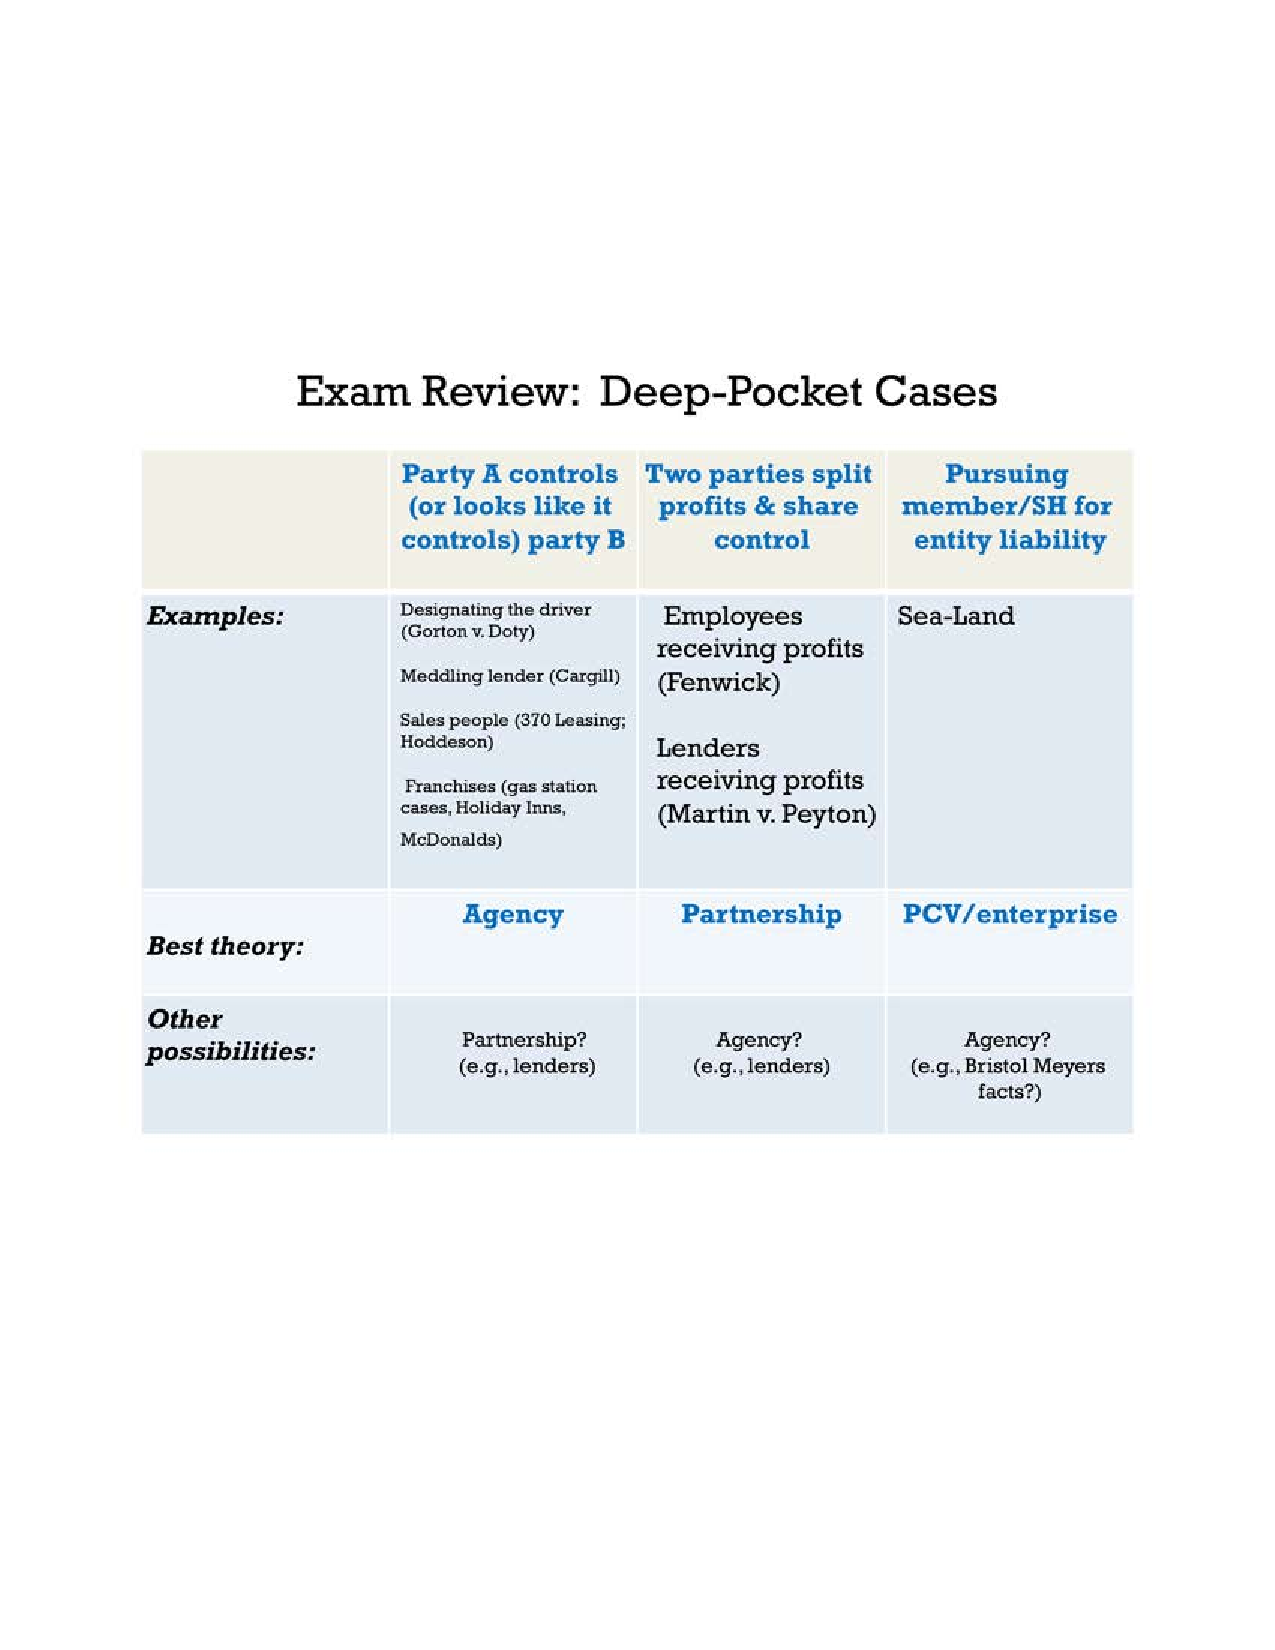
\includepdf{resources/deep-pockets.pdf}
        \end{enumerate}
    \end{enumerate}
    \item \textbf{Role and purpose of the corporation}.
    \begin{enumerate}
        \item Courts are deferential to corporate philanthropy, as long as the 
        corporation avoids \textbf{pet charities}, the donations are 
        \textbf{modest}, and the corporation has a reasonable belief that the 
        donation will \textbf{advance the corporation's interest}. \emph{AP 
        Smith}. % TODO add xref
        \item The donation must have \textbf{some corporate purpose}. You 
        can't just give away money. \emph{Dodge}. % TODO add xref
        \item \textbf{Business judgment rule}: ``Courts will not step 
        in and interfere with honest business judgment of the directors unless 
        there is a showing of fraud, illegality, or conflict of interest.'' 
        \emph{Shlensky v. Wrigley}. % TODO add xref
    \end{enumerate}
\end{enumerate}

\subsection{Limited Liability Company}

\newpage

\begin{enumerate}
    \item \textbf{Limited partnership}:
    \begin{enumerate}
        \item \textbf{Limited} (passive) partners: not personally liable for 
        partnership liabilities.
        \item \textbf{General} (active) partners:
        \begin{enumerate}
            \item Personally liable.
            \item \textbf{At least one required}.
            \item Can be an entity---e.g., VC funds are sometimes organized as 
            LPs with an LLC as the general partner.
        \item Whether someone is a limited or general partner depends on the 
        level of active involvement---e.g., selecting crops to plant, 
        overruling the general partner, signing checks, firing a manger. 
        \emph{Holzman v. De Escamilla}. % TODO add xref
        \end{enumerate}
    \end{enumerate}
    \item \textbf{Limited liability partnership}:
    \begin{enumerate}
        \item Formation: file with the state.
        \item Management rights: partners have the rights of general partners 
        (not passive partners).
        \item Liability: some states limit liability for torts only (not 
        contracts).
        \item Eligibility: professional services (engineers, lawyers, etc.).
    \end{enumerate}
    \item \textbf{Limited liability company}:
    \begin{enumerate}
        \item \textbf{Overview}:
        \begin{enumerate}
            \item \textbf{Nutshell}: Tax advantages of a partnership; limited 
            liability of a corporation; management structure somewhere in 
            between.
            \item \textbf{History}: introduced in late 70s, tax status settled 
            in late 90s.
            \item \textbf{Tax}:
            \begin{enumerate}
                \item \textbf{No double taxation} on operating profits and 
                losses; they \textbf{flow through} to owners.
                \item Easy for an LLC to convert to a corporation, but not the 
                other direction because of the \textbf{tax trap}.
            \end{enumerate}
            \item \textbf{S-corporation}:
            \begin{enumerate}
                \item Regular corporation under state statutes, but with 
                special IRS paperwork.
                \item \textbf{Flow-through} taxation.
                \item 100 shareholder limit.
                \item Entities can't own shares.
                \item No preferred stock.
                \item For the last three reasons, \textbf{VCs disfavor 
                s-corps.}
            \end{enumerate}
            \item \textbf{Formation}:
            \begin{enumerate}
                \item File \textbf{articles of organization}.
                \item Establish \textbf{operating agreement}.
            \end{enumerate}
            \item \textbf{Membership}:  
            \begin{enumerate}
                \item \textbf{Owners} are ``members.''
                \item Default financial structure is similar to that of a 
                partnership.
            \end{enumerate}
            \item \textbf{Management}:
            \begin{enumerate}
                \item \textbf{Member-managed} (default rules):
                \begin{itemize}
                    \item Equal management rights.
                    \item Majority vote decides most matters.
                    \item Unanimity required for extraordinary matters (e.g., 
                    merger, dissolution).
                    \item Operating agreements often modify the default rules.
                \end{itemize}
                \item \textbf{Manager-managed}:
                \begin{itemize}
                    \item Multiple managers allowed.
                    \item Equal management rights.
                    \item Majority manager vote decides most issues.
                    \item Majority \emph{member} vote required for 
                    extraordinary matters.
                    \item Managers don't have to be members.
                \end{itemize}
            \end{enumerate}
            \item \textbf{Transferability}:
            \begin{enumerate}
                \item Similar rules to those in partnership.
                \item Members can assign their \textbf{economic} interest. 
                \item Admission of new members requires consent of all other 
                members.
                \item Operating agreements usually have buyout and buy-sell 
                provisions.
            \end{enumerate}
            \item \textbf{Fiduciary duties}: see below.
            \item \textbf{Limited liability}:
            \begin{enumerate}
                \item Limited under ULLCA \S\ 303(a).
                \item Veil can be pierced---see below.
            \end{enumerate}
        \end{enumerate}
        \item \textbf{Operating agreements}:
        \begin{enumerate}
            \item Indicate whether \textbf{member-managed or manager-managed}.
            \item Change \textbf{management rights} (the default is equal 
            rights under ULLCA \S\ 404).
            \item Change which members are \textbf{agents} (default: all are; 
            ULLCA \S\ 301). Each member in a member-managed LLC has 
            \textbf{statutory apparent authority} to bind the LLC for 
            ``business of the kind'' that the LLC engages in. ULLCA \S\ 301.
        % TODO elf v jaffari
        % TODO fisk v segal
        \end{enumerate}
        \item \textbf{Piercing the LLC veil}---generally the same as PCV. See 
        ULLCA \S\ 303(b) on formalities. Veil can be pierced when:
        \begin{enumerate}
            \item \textbf{Unity of interest and ownership}:
            \begin{itemize}
                \item Lack of formalities.
                \item Commingling of funds or assets.
                \item Under-capitalization.
            \end{itemize}
            \item \textbf{Injustice}:
            \begin{itemize}
                \item Fraud-like conduct.
                \item Unjust enrichment.
            \end{itemize}
        % TODO kaycee
        \end{enumerate}
        \item \textbf{Fiduciary duties}:
        \begin{enumerate}
            \item \textbf{Member-managed}:
            \begin{enumerate}
                \item All members have duties of loyalty and care.
            \end{enumerate}
            \item \textbf{Manager-managed}:
            \begin{enumerate}
                \item Managers have duties of care and loyalty.
                \item Members have no duties in their role as members.
            \end{enumerate}
        % TODO mcconnell
        \end{enumerate}
    \end{enumerate}
\end{enumerate}
